% Compact PGFPlots panel for sampled qldpc_46_2_5_cluster_variant43_cap6 BSC correction-class derivative.
% Requires \usepackage{pgfplots} and \pgfplotsset{compat=1.18}.
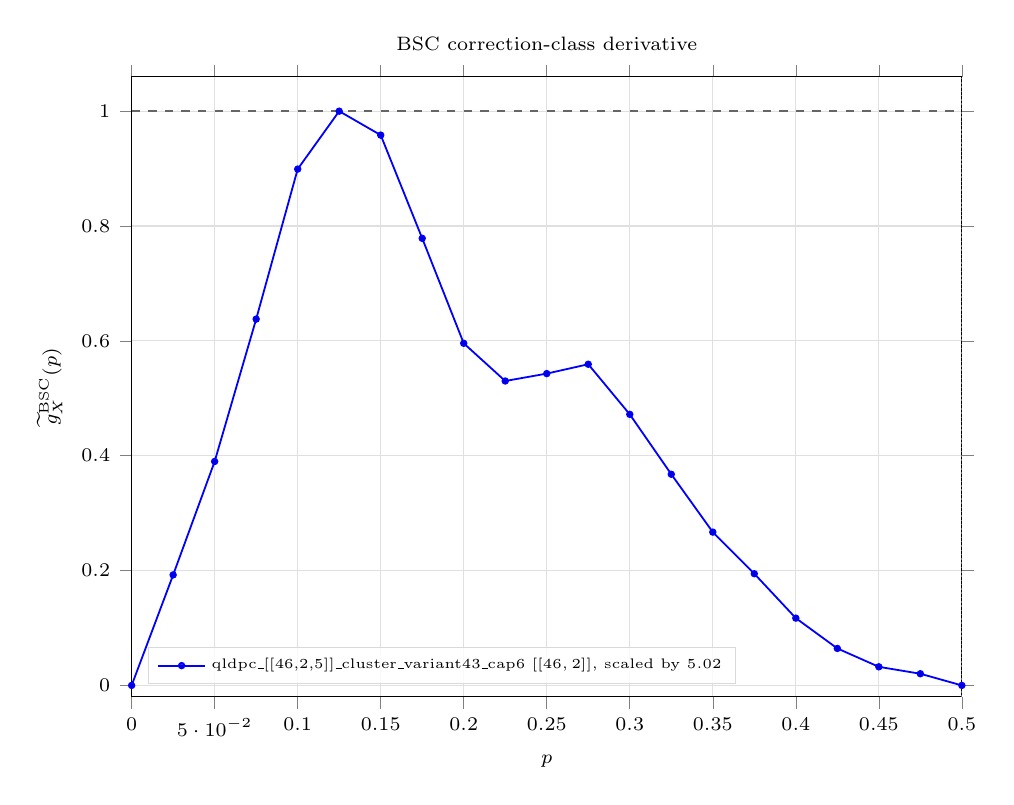
\begin{tikzpicture}
\begin{axis}[
  name=scaledBSCGEXITQldpc4625ClusterVariant43Cap6Axis,
  width=\linewidth,
  height=0.78\linewidth,
  title={BSC correction-class derivative},
  title style={font=\scriptsize},
  xlabel={$p$},
  ylabel={$\widetilde g_X^{\rm BSC}(p)$},
  xmin=0, xmax=0.5,
  ymin=-0.02, ymax=1.06,
  grid=both,
  major grid style={black!12},
  minor grid style={black!6},
  tick align=outside,
  tick label style={font=\scriptsize},
  label style={font=\scriptsize},
  legend cell align={left},
  legend style={draw=black!15, fill=white, fill opacity=0.82, text opacity=1, at={(0.02,0.02)}, anchor=south west, font=\tiny},
]
\addplot[black!60, densely dotted, line width=0.55pt, forget plot] coordinates {(0.5,-0.02) (0.5,1.06)};
\addplot[black!60, dashed, line width=0.55pt, forget plot] coordinates {(0,1) (0.5,1)};
\addplot+[color=blue, mark=*, mark size=1.0pt, line width=0.65pt]
coordinates {(0,0) (0.025,0.192446726061) (0.05,0.390005768675) (0.075,0.637941068259) (0.1,0.899137871725) (0.125,1) (0.15,0.958334866562) (0.175,0.778579233531) (0.2,0.595763316715) (0.225,0.530128993322) (0.25,0.543001559064) (0.275,0.559307024661) (0.3,0.472030975956) (0.325,0.367745592798) (0.35,0.266951273897) (0.375,0.194520235755) (0.4,0.117210955421) (0.425,0.064403090981) (0.45,0.0324085373936) (0.475,0.0203475899661) (0.5,0)};
\addlegendentry{qldpc\_[[46,2,5]]\_cluster\_variant43\_cap6 $[[46,2]]$, scaled by $5.02$}
\end{axis}
\end{tikzpicture}
